% this file is called up by thesis.tex
% content in this file will be fed into the main document

%: ----------------------- name of chapter  -------------------------
\chapter{Your Contribution} % top level followed by section, subsection

In Chapter 2 multiple alternatives to automating authentication were discussed. This section will focus on the solution developed as part of this theses. 


%: ----------------------- paths to graphics ------------------------

% change according to folder and file names
\ifpdf
    \graphicspath{{X/figures/PNG/}{X/figures/PDF/}{X/figures/}}
\else
    \graphicspath{{X/figures/EPS/}{X/figures/}}
\fi

%: ----------------------- Mobile Cloud Middleware ------------------------

\section{Short description of the solution}
This solution is not an application being installed on a device, but is a library that developers can apply in their applications with very little coding. All needed to do is import the library into a project and refer to it.

The library provides easy registration for new credentials, storing them and retrieving for authentication. The user only inserts the credentials once and protects them with a pattern which is used for retrieving them. The pattern and the credentials are stored locally in a database, which is application specific and can only be accessed by it. 

An exapmle project is used in this paper for demonstation puproses.

\newpage

\section{Android lockpattern}
\begin{wrapfigure}{r}{0.4\textwidth} 
\begin{center} 
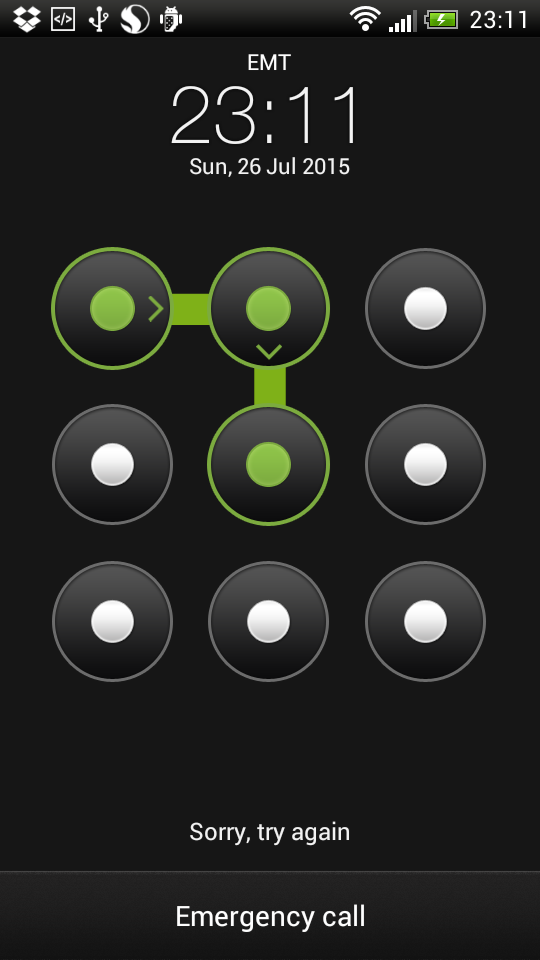
\includegraphics[width=0.35\textwidth]{images/lockpattern.png} \caption{Android lockpattern} \label{fig:android lockpattern} 
\end{center}
\end{wrapfigure}
As mentioned in the previous section a pattern is used to protect the credentials. Android users might already be familiar with the lockpattern even when they have not heard the term itself. It is used for locking the device from unwanted access to it, shown in the Figure 4.1. It is a 3x3 matrix consisting of circles/dots. To draw a pattern a user must press on a circle and drag through others to make a pattern and release to verify it. Even though the user only sees a picture of the pattern it is actually a string of numbers representing the dots where the user changed direction. For example a string "1-7-8" would be a pattern "L". 
Android lockpattern is known to users and is very easy to understand. Typing is taken out of the authentication process, which reduces the amount of errors made, and therefore used in this solution.

\section{Supporting Multiple Users}
The key factor what makes it different from previous solutions is the support for multiple users. Credentials for user authentication is kept in a local database accessed only by the application.

\section{Summary}
Summarize the chapter with at least two paragraphs.



% ---------------------------------------------------------------------------
%: ----------------------- end of thesis sub-document ------------------------
% ---------------------------------------------------------------------------

